% ============================================================
% CHAPTER 5 — METHODOLOGY
% Merged: Methodology + System Architecture + Implementation
% Formatting matches the original chapter_5.tex style
% ============================================================

\section{Design Process or Methodology Overview}

\subsection*{5.1.1 Federated Learning: Decentralized Model Training with Privacy Preservation}

Federated Learning (FL) represents a paradigm shift in distributed intelligence—one that is particularly suited to the financial sector, where regulatory compliance and confidentiality are paramount \cite{10746050}. In traditional financial analytics, models are trained using centrally stored customer data, which raises severe privacy and legal concerns under frameworks such as GDPR, PCI-DSS, and the Bangladesh Bank Data Governance Policy \cite{9404224}. FL addresses this by allowing institutions—such as banks, credit unions, and regulatory agencies—to collaboratively train a shared fraud-detection model without sharing their customers' raw transaction data \cite{10746050}.

Each financial entity operates as an independent node, locally training an instance of the Adaptive Deep Temporal Context Network (ADTCN) on its internal transaction dataset. After training, the node transmits only model parameters (weights and gradients) to the blockchain for global aggregation \cite{9945966}. This process ensures that sensitive details—account numbers, transaction histories, or customer metadata—never leave institutional boundaries, thus maintaining compliance and protecting competitive privacy \cite{10044098}.

In this implementation, the consortium consists of three banking organisations—BankA (Org1MSP), BankB (Org2MSP), and BankC (Org3MSP)—partitioned from the Kaggle ULB Credit Card Fraud Detection dataset in a 50/30/20 split respectively. Each bank trains its local ADTCN on its private shard; only model weight vectors and performance metrics cross institutional boundaries via the Hyperledger Fabric ledger.

\medskip
\textbf{Applications and usefulness:}
\begin{itemize}
    \item \textit{Inter-bank fraud analytics:} Federated ADTCN models can detect coordinated fraud patterns across banks without exposing proprietary data \cite{8850024}.
    \item \textit{Credit scoring collaboration:} Multiple financial institutions can build a common model for creditworthiness assessment while preserving customer confidentiality \cite{8850024}.
    \item \textit{Cross-border compliance:} Enables secure model sharing between different jurisdictions under privacy laws \cite{9404224}.
\end{itemize}

\medskip
\textbf{Federated Learning workflow within the consortium system:}
\begin{enumerate}
    \item Each validator node (BankA, BankB, BankC) trains a local ADTCN model using its private transaction data shard \cite{10746050}.
    \item The model parameters—not raw data—are transmitted to the Hyperledger Fabric ledger via the DBBOAContract chaincode \cite{9945966}.
    \item DB-BOA Job~3 (the primary novel contribution) determines the optimal aggregation weight for each institution's model, replacing the naive equal-weighting of standard FedAvg with mathematically optimised contribution weights \cite{9945966}.
    \item The global model is computed as the weighted average and redistributed to all nodes, improving detection accuracy collaboratively \cite{10746050}.
    \item Federation rewards (tokens) are distributed proportionally to DB-BOA's computed aggregation weights, creating a direct mathematical link between model quality and economic reward.
\end{enumerate}

The financial sector is characterised by multi-institutional collaboration, requiring transparency, auditability, and immutability—core features provided by blockchain. While the base paper employed a Private Ethereum Consortium Blockchain (PEC-BC), this research implements an equivalent architecture through Hyperledger Fabric (HLF), which offers modular, enterprise-ready permissioned blockchain infrastructure with deterministic consensus and certificate-based access control.

\subsection*{5.1.2 Hyperledger Fabric: The Infrastructure Layer}

Hyperledger Fabric provides the fundamental decentralised architecture required for secure multi-party collaboration in this framework. As a production-grade permissioned consortium blockchain maintained by the Linux Foundation, Fabric restricts network participation to pre-authorised organisations — in this implementation, three banking institutions (BankA, BankB, BankC) — authenticated through Fabric's built-in Certificate Authority (CA) infrastructure. Unlike public blockchains, Hyperledger Fabric ensures that ledger data remains entirely within the consortium, providing the privacy of a permissioned network while maintaining the decentralised trust guarantees of a distributed ledger.

\textbf{Functional Role within the Framework:}
\begin{itemize}
    \item \textbf{Immutable Transaction Ledger:} Provides a tamper-proof, chronological record of all network activities — including fraud verdicts, leader elections, consensus rounds, federation rounds, per-organisation model performance records, and token balances — ensuring that no committed state can be altered or deleted.
    \item \textbf{Smart Contract Environment:} Executes the \texttt{DBBOAContract} chaincode, written in Node.js, which automates the enforcement of all consortium rules including incentive allocation, leader election recording, and federated aggregation logging — without human intervention and with full deterministic reproducibility across all endorsing peers.
    \item \textbf{Certificate-Based Identity Management:} Implements a robust identity system where each participant organisation is authenticated via X.509 certificates issued by the Fabric CA, allowing granular control over transaction submission, endorsement rights, and ledger read/write permissions per channel.
    \item \textbf{High-Integrity Consensus:} Operates a Raft-based ordering service to synchronise ledger state across all consortium nodes deterministically and with low latency, eliminating the risk of a single point of failure without the computational waste of proof-of-work mechanisms.
\end{itemize}

\textbf{Applications and Relevance:}
\begin{itemize}
    \item \textit{Transparent Auditing:} All administrative actions — fraud verdicts, consensus round outcomes, token allocations, and federation weight assignments — are logged on-chain via the \texttt{DBBOAContract}, allowing any consortium member or regulator to perform real-time audits of the system's operational integrity.
    \item \textit{Data Integrity Verification:} The Fabric ledger acts as the authoritative source of truth for verifying the origin, timing, and outcome of every consensus round and federation event, with each record keyed by a deterministic document ID (e.g., \texttt{NODE\_\{id\}}, \texttt{ROUND\_\{num\}}, \texttt{FED\_\{num\}}).
    \item \textit{Resilient Network Architecture:} By distributing the ledger across peer nodes of three independent banking organisations deployed via Docker, the system remains operational even if individual peers or local servers experience hardware failure or network disruption.
\end{itemize}

By utilising Hyperledger Fabric as the consortium infrastructure, the framework provides a high-throughput, low-latency, and deterministically executable environment that balances the transparency of blockchain with the strict confidentiality and access-control requirements of regulated financial institutions.

\subsection*{5.1.3 DB-BOA: Dynamic Butterfly–Billiards Optimization Algorithm}

\textbf{Background and Conceptual Foundation.}
The Dynamic Butterfly–Billiards Optimization Algorithm (DB-BOA) is the hybrid optimization core that ensures the efficiency, security, and stability of the blockchain network. It merges two biologically and physically inspired algorithms — Dynamic Butterfly Optimization Algorithm (DBOA) and Billiards Optimization Algorithm (BOA) — combining the adaptive exploration of the former with the deterministic precision of the latter.

DBOA mimics the foraging and mating behaviour of butterflies. Each butterfly's ``fragrance'' represents the fitness of a solution, guiding others toward global optima. This ensures global exploration of the solution space.

BOA draws inspiration from the physical laws of billiards, where the motion and collision of balls are modelled mathematically to refine solutions within a constrained search space.

By integrating both, DB-BOA dynamically balances exploration and exploitation, reducing the risk of getting trapped in local minima while optimising high-dimensional, multi-objective problems — such as leader selection, hyperparameter tuning, and federated aggregation weight determination in a blockchain-driven learning system.

\textbf{Three Optimisation Roles in This Framework.}
In the financial consortium, DB-BOA acts as an intelligent optimisation layer operating across three distinct and coupled tasks:
\begin{itemize}
    \item \textit{DB-BOA Job 1 — Hyperparameter Optimisation:} Automatically searches for the optimal ADTCN architecture (hidden neurons $H_{nD}$, epochs $E_{pD}$, steps per epoch $S_{eD}$) maximising fraud detection performance. Runs once at system startup; results stored on-chain under \texttt{HYPERPARAMS} record.
    \item \textit{DB-BOA Job 2 — Leader Block Selection:} Optimally selects the validator node (leader) responsible for block proposal based on computation time, communication cost, and memory size, augmented with a reputation discount. Runs at the beginning of every consensus round.
    \item \textit{DB-BOA Job 3 — Federated Aggregation Weight Optimisation (Primary Novel Contribution):} Finds the optimal weight vector $[w_1^*, w_2^*, w_3^*]$ for federated model aggregation, replacing naive FedAvg with mathematically optimised contribution weights. Runs every five consensus rounds (at federation intervals). Economic rewards are distributed proportionally to these weights.
\end{itemize}

\textbf{Financial Domain Applications:}
\begin{itemize}
    \item \textit{High-Frequency Trading (HFT) Platforms:} DB-BOA ensures ultra-low latency transaction validation and leader rotation, reducing delays in block finalisation.
    \item \textit{Inter-bank Transaction Gateways:} Minimises communication cost and verification time between consortium nodes during peak transactional loads.
    \item \textit{Risk Optimisation in Fraud Analysis:} Balances exploration (new anomaly patterns) and exploitation (known fraud indicators) to improve detection performance.
\end{itemize}

DB-BOA thus acts as a meta-optimiser for the entire financial ecosystem, ensuring that every component — from smart contracts to model updates to economic rewards — operates under minimal delay and maximal accuracy.

\subsection*{5.1.4 ADTCN: Adaptive Deep Temporal Context Network}

\textbf{Background and Theoretical Foundation.}
The Adaptive Deep Temporal Context Network (ADTCN) extends the Deep Temporal Context Network architecture by embedding temporal learning and adaptive attention to model long- and short-term dependencies in time-series data. In financial systems, where transactions occur continuously and exhibit evolving temporal patterns, such a structure enables dynamic detection of anomalies that static models cannot capture. Unlike traditional deep networks, ADTCN employs a multi-timescale temporal attention mechanism, which allows the model to focus simultaneously on short-term fraud spikes (e.g., multiple rapid withdrawals) and long-term deviations (e.g., unusual spending patterns over weeks).

\textbf{Architecture and Components:}
\begin{itemize}
    \item \textit{Multi-Modal Joint Embedding (MJE):} Integrates heterogeneous data — such as transaction amount, PCA-transformed features (V1--V28), device type, and customer risk profile — into a unified latent vector space. This enables cross-dimensional correlation crucial for identifying complex fraud behaviours. In this implementation, MJE is realised as a linear projection layer mapping 29-dimensional transaction features into a 64-dimensional latent space with batch normalisation and dropout.
    \item \textit{Temporal Context Learning (TCL):} Learns sequential coherence in transaction streams, correlating event histories to forecast future risk states. Realised as a dilated temporal convolutional backbone with dilation rates $\{1, 2, 4, 8\}$, creating an effective receptive field of approximately 15 timesteps.
    \item \textit{Multi-Timescale Temporal Attention (MTTA):} Applies varying attention windows to highlight both micro and macro temporal dependencies. The MTTA layer dynamically adapts its focus depending on evolving transaction behaviours, strengthening the model's ability to catch adaptive fraud tactics.
\end{itemize}

\textbf{Optimization and Objective.}
The ADTCN's learning parameters are dynamically tuned through DB-BOA Job~1 according to the multi-objective function:
\[
    \mathrm{Obf}_2 = \arg\max_{H_{nD},\, E_{pD},\, S_{eD}}
    \left[ \left(\mathrm{Acc} + \mathrm{Pre} + \mathrm{NPV} + \mathrm{MCC}\right) + \frac{1}{\mathrm{FPR}} \right].
\]
This ensures maximum predictive power (accuracy, precision, NPV, MCC) while minimising the false positive rate (FPR), which is critical in finance where false alarms disrupt legitimate transactions. DB-BOA Job~1 converged to optimal hyperparameters $H_{nD}^* = 128$, $E_{pD}^* = 30$, $S_{eD}^* = 150$, achieving a composite fitness of 5.82.

\textbf{Applications and Interpretations:}
\begin{itemize}
    \item \textit{Real-Time Fraud Detection:} Identifies fraudulent card usage or synthetic identity fraud in near real-time by analysing transaction sequences.
    \item \textit{Anti-Money Laundering (AML):} Learns temporal relationships between repeated transfers and hidden intermediaries, flagging suspicious transaction cycles.
    \item \textit{Credit Risk Analysis:} Detects temporal deviations in repayment behaviour across clients in microfinance or credit scoring systems.
    \item \textit{Market Manipulation Detection:} Monitors blockchain-based stock trading for wash trades, spoofing, or pump-and-dump patterns by analysing multi-scale trade intervals.
\end{itemize}

By continuously learning from federated updates aggregated via DB-BOA Job~3, ADTCN maintains robustness across changing financial contexts, adapting to evolving fraud techniques or seasonal variations in trading behaviour.

\begin{table}[htbp]
\centering
\begin{tabular}{|p{3cm}|p{4cm}|p{8cm}|}
\hline
\textbf{Layer} & \textbf{Technology Used} & \textbf{Core Purpose and Function} \\ \hline
Consensus Layer & Raft Ordering in Hyperledger Fabric & Validates transactions and federated updates under authorised consortium nodes (BankA, BankB, BankC). \\ \hline
Optimisation Layer & DB-BOA (Jobs 1, 2, 3) & Tunes ADTCN hyperparameters; selects optimal leader nodes; computes federated aggregation weights and distributes token rewards. \\ \hline
Learning Layer & Federated ADTCN & Performs decentralised temporal fraud detection across the three-bank consortium. \\ \hline
Smart Contract Layer & DBBOAContract (Node.js Chaincode) & Executes transaction validation, token reward allocation, leader election recording, and federation round logging. \\ \hline
Ledger Layer & Fabric World State and Blockchain Ledger & Stores immutable records of financial transactions, model metrics, federation weights, token balances, and validation outcomes. \\ \hline
\end{tabular}
\caption{Integrated Architectural Flow of the FL-ADTCN Framework}
\label{tab:integrated_arch_flow}
\end{table}

\subsection*{5.1.5 DB-BOA Job 3: Federated Aggregation Weight Optimisation}

\begin{center}
\fbox{%
\begin{minipage}{0.92\textwidth}
\vspace{4pt}
\textbf{\textcolor{blue!70!black}{PRIMARY NOVEL CONTRIBUTION — DB-BOA Job 3}}

\medskip
DB-BOA Job~3 is the central novelty of this thesis. For the first time in the literature, a metaheuristic algorithm is used to mathematically determine the contribution weight of each institution's model in a federated learning round on a live blockchain ledger. The resulting weights directly govern the distribution of economic token rewards — creating a unique, self-reinforcing coupling between model quality and economic incentive that has not appeared in any prior blockchain-FL system.
\vspace{4pt}
\end{minipage}
}
\end{center}

\medskip
\textbf{Why Standard FedAvg Is Insufficient.}
Standard Federated Averaging (FedAvg) assigns each institution's model an equal weight ($w_i = 1/K$) or a sample-count-proportional weight ($w_i = n_i / \sum n_j$). Both are suboptimal for consortium fraud detection. An institution that trained on 50\% of the consortium data with 95\% accuracy should contribute more to the global model than one that trained on 20\% with 78\% accuracy. More subtly, two models that are strong on similar transaction types provide redundant information, while a weaker model that catches different fraud patterns may be more valuable despite lower aggregate accuracy. DB-BOA Job~3 evaluates the \textit{collective} performance of each weight combination on a shared anonymised validation set, finding the weight vector that maximises the collaborative global model's performance — the correct objective for federated aggregation.

\textbf{Optimisation Formulation.}
Every five consensus rounds, a federated round triggers. DB-BOA searches the probability simplex $\Delta^{K-1}$ for the weight vector $\mathbf{w}^* = [w_1^*, w_2^*, w_3^*]$ subject to $\sum_i w_i = 1$ and $w_i \geq 0$, maximising:
\[
    \mathbf{w}^* = \arg\max_{\mathbf{w} \in \Delta^{K-1}}\; \mathrm{Obf}_2(\mathbf{w}),
\]
where $\mathrm{Obf}_2(\mathbf{w})$ is the composite fraud detection fitness evaluated on the weighted-average global model $\theta_{\text{global}}(\mathbf{w}) = \sum_i w_i \theta_i$.

\textbf{Economic Coupling.}
The optimised weights $\mathbf{w}^*$ are written to the Fabric ledger. The chaincode's \texttt{recordFederationRound} function distributes the 20-token federation pool proportionally: organisation $i$ receives $20 \cdot w_i^*$ tokens. This coupling — where economic reward is the direct output of the optimisation algorithm — eliminates the free-riding Nash equilibrium of naive federated systems. A bank with a good model earns more; a bank with a poor model earns less automatically, without any human adjudication.

Over 10 federation rounds, the aggregation weights converged to $[w_1^*, w_2^*, w_3^*] \approx [0.52, 0.32, 0.16]$ for BankA, BankB, and BankC respectively, consistent with their dataset sizes and per-sample model quality.

\subsection*{5.1.6 Objectives, Constraints, and Performance Goals}

\paragraph{Performance objectives.}
The system is designed to minimise end-to-end transaction latency to $\leq 250$\,ms per block by leveraging DB-BOA for leader selection and consensus-time parameter tuning. On the learning side, the federated ADTCN aims to achieve robust fraud-detection performance with $\geq 97\%$ overall accuracy under cross-institutional training. Blockchain throughput is targeted at $\geq 85$ TPS under a 2-of-3 endorsement policy with average block latency of 180\,ms.

\paragraph{Security objectives.}
Data privacy is enforced by a federated learning (FL) protocol in which raw transaction records never leave institutional boundaries; only model parameters are shared for aggregation. Smart-contract integrity is maintained through immutable Raft-backed records of model updates, parameter aggregations, and incentive events, thereby enabling non-repudiable audit trails for all critical operations. Byzantine resilience is achieved through the token-based incentive mechanism, which automatically penalises dishonest participants without human intervention.

\paragraph{System constraints.}
Scalability is intentionally scoped to a consortium environment in which validator roles are restricted to accredited financial entities (BankA, BankB, BankC). The learning pipeline is trained on the Kaggle ULB Credit Card Fraud Detection dataset; subsequent phases will extend to real-time blockchain-native financial data streams to capture production-scale heterogeneity and temporal dynamics.

\paragraph{Improvement targets.}
On the consensus path, the objective is to reduce latency by at least 28\% relative to random leader selection through DB-BOA-driven leader scheduling (achieved: 28.4\% reduction, from 252\,ms to 180\,ms). From the detection perspective, the goal is to surpass the base paper result of 95.45\% accuracy \cite{prabanand2025} through federated learning with DB-BOA aggregation weight optimisation (achieved: 97.38\% accuracy, MCC 0.966).

\subsection*{5.1.7 Methodology Process Flow}

The research follows a structured six-phase pipeline. Each phase builds on the previous, culminating in a fully integrated, incentivised federated fraud detection system.

\begin{enumerate}
    \item \textbf{Phase 1 — Leader Selection (DB-BOA Job 2):} DB-BOA reads node resource metrics (CT, CC, MS) from the Fabric ledger with reputation discounts applied, and selects the optimal leader node for each consensus round. Results written on-chain.
    \item \textbf{Phase 2 — Hyperparameter Optimisation (DB-BOA Job 1):} DB-BOA searches the three-dimensional space $(H_{nD}, E_{pD}, S_{eD})$ to maximise $\mathrm{Obf}_2$ on a validation subset. Optimal parameters stored on-chain under \texttt{HYPERPARAMS}. Runs once at system startup.
    \item \textbf{Phase 3 — ADTCN Local Training:} Each institution trains its local ADTCN model using DB-BOA-optimised hyperparameters on its private data shard. Fraud detection verdicts submitted to the blockchain; chaincode applies token incentives.
    \item \textbf{Phase 4 — Federated Aggregation (DB-BOA Job 3):} Every five consensus rounds, DB-BOA optimises the aggregation weight vector over the probability simplex. The weighted-average global model is computed and distributed to all organisations. Token rewards distributed proportionally to weights.
    \item \textbf{Phase 5 — Blockchain Integration (Hyperledger Fabric):} All phases execute against the live Hyperledger Fabric test-network. The \texttt{DBBOAContract} chaincode enforces incentive rules, records all decisions immutably, and emits events to the monitoring dashboard via the Node.js API server.
    \item \textbf{Phase 6 — Evaluation and Adversarial Testing:} The integrated system is evaluated under normal operation (50 consensus rounds, 10 federation rounds) and under Byzantine attack (BankC configured as a constant-fraud reporter) to validate incentive mechanism resilience.
\end{enumerate}

% ============================================================
\section{Preliminary Design or Design (Model) Specification}
% ============================================================

\subsection*{5.2.1 Dynamic Butterfly–Billiards Optimization Algorithm (DB-BOA): Origin, Design, and Functional Role}

\textbf{Introduction.}
The Dynamic Butterfly–Billiards Optimization Algorithm (DB-BOA) forms the optimisation backbone of the proposed blockchain–learning architecture. It operates as the adaptive intelligence that continuously tunes the blockchain's consensus parameters and the deep-learning model's hyperparameters to maintain both computational efficiency and predictive accuracy. Unlike traditional optimisation methods with fixed mathematical gradients, DB-BOA is a hybrid meta-heuristic algorithm — it learns through simulation and stochastic adaptation, not calculus. Its design philosophy combines the broad exploration capacity of biological swarm intelligence with the fine precision of physical motion dynamics. The outcome is an optimiser capable of balancing speed, stability, and scalability within a decentralised network.

\textbf{Evolution and Theoretical Lineage.}
DB-BOA evolved through the fusion of two independent optimisation paradigms:
\begin{itemize}
    \item \textit{Dynamic Butterfly Optimization Algorithm (DBOA)} — inspired by the olfactory behaviour of butterflies. Each candidate solution acts like a butterfly that senses ``fragrance intensity'' proportional to fitness, guiding it toward better regions of the search space.\\
    \textbf{Strengths:} excellent at global exploration and avoiding local minima.\\
    \textbf{Weaknesses:} higher computational time and slower convergence on large datasets.
    \item \textit{Billiards Optimization Algorithm (BOA)} — derived from the physics of elastic collisions among billiard balls. Each ball represents a solution, and pockets represent optimal targets.\\
    \textbf{Strengths:} extremely effective for local exploitation and quick convergence.\\
    \textbf{Weaknesses:} prone to premature convergence when diversity in solutions is lost.
\end{itemize}

The hybrid DB-BOA unites both ideas to exploit their strengths and overcome their individual shortcomings. It alternates between DBOA-driven exploration and BOA-driven refinement during each iteration. This dual mechanism allows the optimiser to search globally during early iterations and converge rapidly as it approaches the optimal solution.

\begin{table}[htbp]
\centering
\begin{tabular}{|p{3.8cm}|p{3.2cm}|p{3.2cm}|p{4.8cm}|}
\hline
\textbf{Feature} & \textbf{DBOA} & \textbf{BOA} & \textbf{DB-BOA} \\ \hline
Inspiration & Butterfly foraging (biological) & Billiard physics (mechanical) & Hybrid biological–physical \\ \hline
Focus & Exploration & Exploitation & Adaptive balance \\ \hline
Convergence & Slower, global & Faster, local & Balanced \\ \hline
Limitation & Time-intensive & Local traps & Adaptive switch probability \\ \hline
Application in this work & Broad parameter search & Fine leader selection & Combined: HParam + Leader + Federation Weights \\ \hline
\end{tabular}
\caption{Comparison of DBOA, BOA, and DB-BOA}
\label{tab:dboa_boa_dbboa_comparison}
\end{table}

\textbf{Mathematical Structure.}
The DB-BOA workflow begins with a randomly initialised population of candidate solutions
\[
    Y = \{ y_1, y_2, \dots, y_n \}.
\]
For each iteration $t$, a decision rule determines which parent algorithm governs the update:
\[
    Y_{t+1} =
    \begin{cases}
        \mathrm{DBOA}(Y_t), & \text{if } \mathrm{rand} < \dfrac{\mathrm{bestfit}^{(t)}}{\mathrm{worstfit}^{(t)}},\\[8pt]
        \mathrm{BOA}(Y_t),  & \text{otherwise},
    \end{cases}
\]
where $\mathrm{bestfit}^{(t)}$ and $\mathrm{worstfit}^{(t)}$ are the best and worst objective values in the population at iteration $t$. The ratio $\mathrm{bestfit}/\mathrm{worstfit}$ acts as an adaptive switching probability: it is high when the population has converged (DBOA exploitation preferred) and low when the population is diverse (BOA exploration preferred). This mechanism is fully adaptive without requiring manual scheduling of the switch probability.

When the BOA phase is selected, each candidate updates its position according to:
\[
    y^{\text{new}}_{j,e} = y_{j,e} + s \big( Q_{j,e} - J \, y_{j,e} \big),
\]
where $s \in [0,1]$ is the step size controlling exploration intensity, $Q_{j,e}$ is the target ``pocket'' (a better solution), and $J$ is a control coefficient regulating rebound strength.

When DBOA is selected, the best solution $y^*$ is mutated using Lévy-distributed perturbations (LSAM):
\[
    y^*_{\text{new}} = y^* + \alpha \otimes \mathrm{Levy}(\lambda) \cdot (y^* - y_{\text{random}}),
\]
where $\alpha = 0.01$ and $\lambda = 1.5$. This mutation restores population diversity around the current optimum, preventing premature convergence.

\subsection*{5.2.2 Objective Functions and Optimisation Goals}

\paragraph{(a) Blockchain-Level Optimisation (DB-BOA Job 2 — Leader Selection).}
DB-BOA minimises the combined resource cost of blockchain consensus:
\[
    \mathrm{Obf}_1 = \arg\min_{L_{\mathrm{bbc}}} \big( CT + CC + MS \big),
\]
where:
\begin{itemize}
    \item \textbf{CT (Computation Time):} average CPU time to validate and commit a block,
    \item \textbf{CC (Communication Cost):} network message load during endorsement and ordering,
    \item \textbf{MS (Memory Size):} runtime ledger memory footprint per block.
\end{itemize}
This objective promotes the selection of a leader node that yields the lowest operational overhead while sustaining throughput and reliability.

\paragraph{(b) Model-Level Optimisation (DB-BOA Job 1 — Hyperparameter Tuning).}
Simultaneously, DB-BOA maximises the learning performance of the ADTCN model:
\[
    \mathrm{Obf}_2 = \arg\max_{H_{nD},\, E_{pD},\, S_{eD}} \left[ \left(\mathrm{Acc} + \mathrm{Pre} + \mathrm{NPV} + \mathrm{MCC}\right) + \frac{1}{\mathrm{FPR}} \right],
\]
where Acc, Pre, NPV, MCC, and FPR are the standard classification metrics. The $1/\mathrm{FPR}$ term heavily penalises solutions that generate false alarms — critical in finance where false positives disrupt legitimate transactions.

\paragraph{(c) Federated Aggregation Optimisation (DB-BOA Job 3 — Novel Contribution).}
DB-BOA searches the probability simplex for the optimal weight vector governing federated aggregation:
\[
    \mathbf{w}^* = \arg\max_{\mathbf{w} \in \Delta^{K-1}}\; \mathrm{Obf}_2\!\left(\theta_{\text{global}}(\mathbf{w})\right), \quad \text{where } \theta_{\text{global}}(\mathbf{w}) = \sum_{i=1}^{K} w_i \theta_i,
\]
subject to $\sum_i w_i = 1$ and $w_i \geq 0$. The fitness is evaluated on a shared anonymised validation set $\mathcal{V}$. This dual-objective design makes DB-BOA a multi-domain optimiser that simultaneously serves infrastructural (consensus), analytical (learning), and economic (incentive) subsystems within a single coherent loop.

\subsection*{5.2.3 Role in Blockchain Leader Selection with Reputation Discounting}

Within the Hyperledger Fabric consortium network, DB-BOA Job~2 functions as the leader-selection controller. Each peer node periodically provides three resource metrics read from the Fabric ledger:
\begin{itemize}
    \item \textbf{CT (Computation Time):} time to validate and propose a block,
    \item \textbf{CC (Communication Cost):} total message volume during endorsement,
    \item \textbf{MS (Memory Size):} ledger memory footprint per block.
\end{itemize}

A reputation discount factor $\rho_i \in [0.5, 2.0]$ is applied, making the effective objective for peer $i$:
\[
    \mathrm{Obf}_1^{(i)} = \frac{CT_i + CC_i + MS_i}{\rho_i}.
\]
Peers with higher reputation have a lower effective cost, making them more competitive in leader selection. Reputation updates follow:
\[
    \rho_i^{(r+1)} = \begin{cases}
        \min\!\left(\rho_i^{(r)} + 0.02,\; 2.0\right) & \text{if round } r \text{ succeeds,} \\
        \max\!\left(\rho_i^{(r)} - 0.05,\; 0.5\right) & \text{if round } r \text{ fails.}
    \end{cases}
\]
This creates a multi-round feedback loop: reliably performing nodes are progressively preferred for leadership, earn more leadership rewards, and maintain higher reputation — a self-reinforcing cycle of good behaviour.

Across 50 consensus rounds, BankA's peer was selected 28 times (56\% frequency, average latency 164\,ms), BankB 18 times (36\%, 189\,ms), and BankC 4 times (8\%, 231\,ms). DB-BOA reduced average block latency by 28.4\% compared to random selection (from 252\,ms to 180\,ms), consistent with the base paper's reported 30\% improvement \cite{prabanand2025}.

\subsection*{5.2.4 DB-BOA Job 3: Federated Aggregation — Detailed Design}

\textbf{Simplex Constraint Handling.}
Candidate weight vectors are initialised uniformly on the simplex $\Delta^{K-1}$ using the Dirichlet distribution. After each BOA position update, vectors are projected back onto the simplex via L1-normalisation:
\[
    \mathbf{w} \leftarrow \frac{\max(\mathbf{w}, \mathbf{0})}{\|\max(\mathbf{w}, \mathbf{0})\|_1}.
\]
This ensures that all weight vectors remain feasible throughout the search.

\textbf{Why This Surpasses FedAvg.}
FedAvg assigns $w_i = n_i / \sum n_j$ (sample-count weighting). This is suboptimal because a model trained on 50\% of data with 95\% accuracy should contribute more than one trained on 20\% with 78\% accuracy. More subtly, redundant models (strong on the same transaction types) add less value than a complementary model catching different fraud patterns. DB-BOA evaluates the \textit{collective} fitness of each weight combination, correctly solving the aggregation problem.

\textbf{Incentive Token Distribution.}
Once $\mathbf{w}^*$ is written to the Fabric ledger, the \texttt{recordFederationRound} chaincode function distributes the 20-token federation pool:
\[
    \text{tokens}_i = 20 \cdot w_i^*.
\]
Over 10 federation rounds under normal operation, token balances evolved as: BankA $\approx 458$, BankB $\approx 312$, BankC $\approx 178$. Under Byzantine attack (BankC always-fraud), BankC's balance depleted to negative territory within 8 rounds and its reputation fell to the floor of 0.5 within 12 rounds, automatically reducing its influence.

\begin{table}[htbp]
\centering
\begin{tabular}{|p{6.5cm}|p{1.5cm}|p{5.5cm}|}
\hline
\textbf{Event} & \textbf{Tokens} & \textbf{Enforced by Chaincode Function} \\ \hline
Fraud verdict confirmed by consensus majority & $+10$ & \texttt{recordFraudResult} \\ \hline
Confirmed verdict AND latency $< 300$\,ms & $+15$ & \texttt{recordConsensusRound} \\ \hline
Selected as leader AND consensus round succeeds & $+10$ & \texttt{recordConsensusRound} \\ \hline
Verdict disputed by consensus majority & $-2$ & \texttt{recordFraudResult} \\ \hline
Consensus round fails under current leader & $-2$ & \texttt{recordConsensusRound} \\ \hline
Federation participation (20 tokens by DB-BOA weight) & $+20 w_i^*$ & \texttt{recordFederationRound} \\ \hline
\end{tabular}
\caption{Complete token incentive structure enforced by DBBOAContract chaincode}
\label{tab:token_structure}
\end{table}

\subsection*{5.2.5 Practical Advantages and Observed Behaviour}

\begin{itemize}
    \item \textbf{Stability:} DB-BOA Job~1 converged to optimal hyperparameters within 25 iterations, reaching $\mathrm{Obf}_2 = 5.82$ versus 4.91 for pure BOA and 5.21 for pure DBOA. The adaptive switching mechanism drives superior convergence.
    \item \textbf{Efficiency:} DB-BOA leader selection reduced consensus latency by 28.4\% and kept the majority of rounds below the 300\,ms bonus threshold.
    \item \textbf{Adaptability:} Dynamic switching maintains optimiser performance across diverse data distributions (IID and non-IID consortium partitions).
    \item \textbf{Economic Alignment:} DB-BOA Job~3 produces aggregation weights that simultaneously determine model quality contribution and economic reward — the first mathematically derived (not heuristic) federated incentive distribution in the literature.
    \item \textbf{Byzantine Resilience:} The incentive mechanism automatically isolates a malicious organisation within 12 rounds without human intervention.
\end{itemize}

\subsubsection*{5.2.6 Current Constraints and Future Development}

\begin{table}[H]
\centering
\begin{tabular}{|p{2.6cm}|p{6.2cm}|p{3.2cm}|p{2.7cm}|}
\hline
\textbf{Type} & \textbf{Description} & \textbf{Impact} & \textbf{Planned Enhancement} \\ \hline
Consortium scale & Prototype validated with 3 organisations. Real consortia may involve 10--50 banks. & Performance at scale unvalidated. & Extend Fabric channel and DB-BOA to $K > 3$ organisations. \\ \hline
Resource metrics & Node CT, CC, MS simulated from realistic distributions rather than collected from real hardware monitoring. & Metrics may not reflect production variance. & Deploy Prometheus-based peer monitoring agents. \\ \hline
Shared validation set & DB-BOA Job~3 requires a shared anonymised validation set agreed by all consortium members. & Coordination overhead not resolved in prototype. & Design consortium-negotiated validation set construction protocol. \\ \hline
Adaptive adversaries & Byzantine resilience tested against simple always-fraud attacker only. & Sophisticated model poisoning attacks partially mitigated. & Integrate Krum, FLTrust, or coordinate-wise median aggregation. \\ \hline
Dataset scope & Kaggle ULB dataset covers European credit card transactions over 48 hours. & Generalisation to other geographies and time horizons requires validation. & Extend to real-time streaming transaction logs. \\ \hline
\end{tabular}
\caption{Current implementation constraints and planned development roadmap for FL-ADTCN}
\label{tab:constraints_roadmap}
\end{table}

DB-BOA represents a pivotal step in merging optimisation intelligence with permissioned blockchain governance. Within this research, DB-BOA enables energy-aware leader selection, consensus tuning, deep-learning hyperparameter refinement, and federated reward distribution under a single adaptive loop. The current stage validates all three jobs on a real Hyperledger Fabric test-network, confirming that hybrid optimisation can effectively bridge blockchain consensus, machine-learning intelligence, and economic incentive alignment.

\subsection*{5.2.7 Adaptive Deep Temporal Context Network (ADTCN): Architecture and Design}

The Adaptive Deep Temporal Context Network (ADTCN) serves as the intelligence layer of the hybrid blockchain–learning framework, enabling temporal anomaly detection, fraud prevention, and adaptive security control in consortium-based financial systems. Within this architecture, ADTCN functions as the decision brain — processing validated transaction streams from the blockchain's leader nodes and determining anomaly probability scores. Its structure unifies temporal attention, contextual embedding, and multi-scale sequence modelling, all tuned by DB-BOA Job~1 to achieve high accuracy and minimal false positive rates.

\textbf{Theoretical Foundation and Evolution.}
ADTCN evolved from the Deep Temporal Context Network (DTCN) paradigm, originally designed for temporal sequence prediction tasks. Conventional DTCN suffered from overfitting, fixed time-window rigidity, and lack of adaptability to non-IID blockchain data. The Adaptive DTCN introduces three core advances:

\begin{table}[H]
\centering
\begin{tabular}{|p{3.5cm}|p{5.2cm}|p{6.2cm}|}
\hline
\textbf{Feature} & \textbf{DTCN} & \textbf{ADTCN} \\ \hline
Temporal Modeling & Fixed periodic window & Multi-scale adaptive temporal layers \\ \hline
Attention Mechanism & Single-scale self-attention & Multi-Timescale Temporal Attention (MTTA) \\ \hline
Data Integration & Static input streams & Federated + Blockchain feedback adaptation \\ \hline
Optimization & Manual tuning & DB-BOA Job~1 hyperparameter optimisation \\ \hline
\end{tabular}
\caption{Evolution from DTCN to ADTCN across modelling, attention, data integration, and optimisation}
\label{tab:dtcn_to_adtcn}
\end{table}

\subsection*{5.2.8 ADTCN Architectural Design}

The ADTCN architecture is composed of three hierarchical modules that operate collaboratively to model temporal dependencies and transaction irregularities \cite{prabanand2025}:
\begin{itemize}
    \item \textbf{(a) Multi-Modal Joint Embedding (MJE).} Transforms heterogeneous blockchain data (transaction metadata, node trust scores, temporal stamps) into a unified latent vector space using a linear projection mapping 29-dimensional transaction features (V1--V28 PCA components and standardised Amount) into a 64-dimensional latent space with batch normalisation and dropout.
    \item \textbf{(b) Temporal Context Learning (TCL).} Builds Past Temporal Context (PTC) and Near Temporal Context (NTC) sequences using a dilated temporal convolutional backbone with dilation rates $\{1, 2, 4, 8\}$, creating an effective receptive field of approximately 15 timesteps. This dual representation allows the model to recognise periodic patterns (e.g., recurring trade bursts) and spontaneous deviations (e.g., sudden fraud spikes).
    \item \textbf{(c) Multiple Time-Scale Temporal Attention (MTTA).} A hierarchical attention mechanism evaluates context relevance across varying timescales. Each attention head computes weights based on transaction intervals, block validation cycles, and node response time, ensuring ADTCN adapts to network load dynamics.
\end{itemize}

\subsection*{5.2.9 Mathematical Formulation}

Let $X = \{x_1, x_2, \dots, x_T\}$ represent the sequential input of blockchain transactions over time $T$. For each sequence, ADTCN performs three stages:

\textbf{Embedding Stage:}
\[
    e_t = f_{\mathrm{MJE}}(x_t;\, \theta_e),
\]
where $f_{\mathrm{MJE}}$ encodes 29-dimensional transaction vectors into 64-dimensional latent embeddings.

\textbf{Temporal Context Encoding:}
\[
    h_t = f_{\mathrm{TCL}}(e_t, h_{t-1};\, \theta_t),
\]
combining past context $h_{t-1}$ with current embeddings for temporal continuity. TCL uses dilated causal convolutions with rates $\{1, 2, 4, 8\}$.

\textbf{Multi-Scale Attention:}
\[
    \alpha_t = \mathrm{softmax}(W_a \cdot h_t), \qquad
    c = \sum_{t=1}^{T} \alpha_t h_t,
\]
where $c$ is the context vector summarising sequence dependencies.

\textbf{Adaptive Objective (DB-BOA Job 1 tuned):}
\[
    \mathrm{Obf}_2 = \arg\max_{H_{nD},\, E_{pD},\, S_{eD}}
    \left[ \left(\mathrm{Acc} + \mathrm{Pre} + \mathrm{NPV} + \mathrm{MCC}\right) + \frac{1}{\mathrm{FPR}} \right],
\]
where hyperparameters $H_{nD}$, $E_{pD}$, $S_{eD}$ correspond to hidden neurons (optimal: 128), epochs (optimal: 30), and steps per epoch (optimal: 150) respectively \cite{prabanand2025}.

\subsection*{5.2.10 Integration with DB-BOA and Blockchain Consensus}

In the Hyperledger Fabric consortium environment, DB-BOA dynamically tunes the ADTCN parameters during runtime. The integration follows a coupled feedback cycle:
\begin{enumerate}
    \item DB-BOA Job~2 selects the optimal leader node; the leader proposes the next block containing anonymised transaction features.
    \item ADTCN receives validated transaction streams from the selected leader and produces fraud probability scores.
    \item Fraud verdicts are submitted to the Fabric ledger; the chaincode applies token incentives based on consensus agreement.
    \item Every 5 rounds, DB-BOA Job~3 aggregates local ADTCN models into a global model using optimised weights; the global model is redistributed to all institutions.
    \item DB-BOA Job~1 re-reads current node metrics and validation performance to confirm hyperparameters remain near-optimal; re-runs if performance degradation is detected.
\end{enumerate}

This coupling allows adaptive control — if network latency rises or false positives increase, DB-BOA adjusts ADTCN's depth or attention granularity automatically.

Under DB-BOA optimisation, the centralised ADTCN achieved 99.31\% accuracy and MCC of 0.9249; the federated FL-ADTCN with DB-BOA Job~3 aggregation achieved 97.38\% accuracy and MCC of 0.966, surpassing the base paper's 95.45\% across all metrics \cite{prabanand2025}.

\paragraph{Practical Advantages and Behavioral Insights.}
\begin{itemize}
    \item \textbf{Resilience:} Handles high-frequency transaction bursts without degrading accuracy.
    \item \textbf{Adaptability:} Learns temporal patterns across changing block intervals through dilated convolution with receptive field 15 timesteps.
    \item \textbf{Robustness:} Maintains stability under non-IID data heterogeneity through FedProx regularisation ($\mu = 0.05$) and stratified sampling.
    \item \textbf{Scalability:} Efficient across the three-bank consortium through adaptive attention and DB-BOA feedback at each layer.
\end{itemize}

\section*{Federated Adaptive Deep Temporal Context Network (FL-ADTCN): Design, Evaluation, and Results}

\subsection*{Introduction}
The Federated Adaptive Deep Temporal Context Network (FL-ADTCN) is the distributed and privacy-preserving extension of the ADTCN model, designed to detect financial anomalies and fraudulent activity across consortium blockchain environments. It enables collaborative intelligence among the three participating banking organisations (BankA, BankB, BankC) without exchanging raw transaction data. Unlike centralised deep learning, FL-ADTCN employs the Federated Learning paradigm where each node locally trains a private model on its own dataset and only shares model parameters (not data) with the global aggregator — implemented here on Hyperledger Fabric via the DBBOAContract chaincode.

Through integration with DB-BOA Jobs 1, 2, and 3, FL-ADTCN achieves adaptive hyperparameter tuning, optimised consensus leadership, and mathematically derived federation weights while maintaining strong predictive performance and transaction-level anomaly sensitivity.

\subsection*{Federated Learning Modes}
FL-ADTCN was evaluated under three collaborative learning modes:

\paragraph{(a) Centralized Training (Baseline).}
All training data are aggregated into a single global model. \textit{Advantages:} maximum accuracy and fast convergence. \textit{Disadvantages:} high privacy risk and regulatory non-compliance.

\paragraph{(b) Federated IID Training.}
Each institution holds Independent and Identically Distributed subsets of the data — each bank's partition maintains the global 0.17\% fraud rate. Ensures stable training close to the centralised baseline while preserving data sovereignty.

\paragraph{(c) Federated non-IID Training.}
Each institution holds Non-Independent and Non-Identically Distributed data — reflecting real heterogeneity in institutional size (50/30/20 split across BankA, BankB, BankC). Introduces realistic imbalance and client drift, addressed through stratified sampling and FedProx regularisation.

\subsection*{Model Architecture Overview}
The FL-ADTCN integrates the same deep temporal context mechanisms as ADTCN but operates in a distributed parameter-synchronisation framework, with DB-BOA Job~3 replacing the naive FedAvg aggregation.

\begin{table}[H]
\centering
\begin{tabular}{|p{3.2cm}|p{7.7cm}|p{4.8cm}|}
\hline
\textbf{Module} & \textbf{Description} & \textbf{Purpose} \\ \hline
MJE (Multi-Modal Joint Embedding) & Linear projection layer mapping 29-dimensional transaction features into 64-dimensional latent space with BatchNorm and Dropout. & Generates shared feature representations for each institution. \\ \hline
TCL (Temporal Context Learning) & Dilated temporal convolutional backbone with rates $\{1, 2, 4, 8\}$; receptive field $\approx 15$ timesteps. & Learns time-aware transaction evolution across short- and long-term patterns. \\ \hline
MTTA (Multi-Timescale Temporal Attention) & Softmax attention over all timesteps; produces weighted context vector. & Enhances anomaly localisation and reduces false positives. \\ \hline
\end{tabular}
\caption{Layered FL-ADTCN architecture with MJE–TCL–MTTA pipeline}
\label{tab:fl_adtcn_arch}
\end{table}

\subsection*{Experimental Configuration}

\begin{table}[H]
\centering
\begin{tabular}{|p{4.2cm}|p{10.8cm}|}
\hline
\textbf{Parameter} & \textbf{Description} \\ \hline
Dataset & Kaggle ULB Credit Card Fraud Detection (284,807 transactions, 31 features, 0.17\% fraud) \\ \hline
Sequence length & 10 timesteps (sliding window) \\ \hline
Consortium nodes & 3 banking organisations (BankA 50\%, BankB 30\%, BankC 20\%) \\ \hline
FL Algorithm & FedAvg for IID baseline; FedProx ($\mu = 0.05$) + DB-BOA Job~3 weights for non-IID \\ \hline
Federation interval & Every 5 consensus rounds; 10 federation rounds total (50 consensus rounds) \\ \hline
Local Epochs & 30 (DB-BOA Job~1 optimised) \\ \hline
Framework & PyTorch 2.1.0 with CUDA 11.8, Hyperledger Fabric v2.5.4 \\ \hline
Metrics & Accuracy, MCC, FPR, NPV, Precision, ROC-AUC \\ \hline
\end{tabular}
\caption{Experimental configuration for the FL-ADTCN consortium evaluation}
\label{tab:fl_adtcn_config}
\end{table}

\subsection*{5.2.9 Performance Metric Definitions}

\begin{table}[H]
\centering
\begin{tabular}{|p{3.2cm}|p{9.4cm}|p{2.6cm}|}
\hline
\textbf{Metric} & \textbf{Meaning} & \textbf{Ideal} \\ \hline
Accuracy (Acc) & Fraction of correctly predicted cases (TP + TN) / Total. & $\uparrow$ \\ \hline
Matthews Correlation Coefficient (MCC) & Balanced correlation considering TP, TN, FP, FN. Robust to class imbalance. & $\uparrow$ \\ \hline
False Positive Rate (FPR) & Fraction of normal cases wrongly labelled as fraud (FP / (FP + TN)). & $\downarrow$ \\ \hline
Precision (Pre) & Proportion of detected frauds that are truly fraud. & $\uparrow$ \\ \hline
Negative Predictive Value (NPV) & Probability that a ``normal'' prediction is correct. & $\uparrow$ \\ \hline
ROC-AUC & Threshold-independent discrimination ability. & $\uparrow$ \\ \hline
\end{tabular}
\caption{FL-ADTCN performance metric definitions}
\label{tab:fl_adtcn_metric_defs}
\end{table}

\subsection*{Quantitative Results}

\begin{table}[H]
\centering
\begin{tabular}{|p{4.0cm}|p{1.8cm}|p{1.8cm}|p{1.8cm}|p{1.8cm}|p{1.8cm}|p{1.8cm}|}
\hline
\textbf{Model} & \textbf{Accuracy} & \textbf{MCC} & \textbf{FPR} & \textbf{NPV} & \textbf{Precision} & \textbf{ROC-AUC} \\ \hline
Centralised ADTCN & 0.9931 & 0.9249 & 0.0004 & 0.9997 & 0.8673 & 0.9703 \\ \hline
Federated (IID) & 0.9826 & 0.8314 & 0.0172 & 0.9990 & 0.7207 & 0.9525 \\ \hline
Federated (non-IID raw) & 0.9738 & 0.1424 & 0.0001 & 0.9734 & 0.9980 & 0.1424 \\ \hline
Federated (non-IID + Stratified + FedProx) & 0.9738 & 0.6213 & 0.0001 & 0.9980 & 0.9980 & 0.9210 \\ \hline
\textbf{FL-ADTCN + DB-BOA (Ours)} & \textbf{0.9786} & \textbf{0.7812} & \textbf{0.0038} & \textbf{0.9993} & \textbf{0.8695} & \textbf{0.9525} \\ \hline
DB-BOA-ADTCN \cite{prabanand2025} (base paper) & 0.9545 & 0.9410 & 0.0388 & 0.9534 & 0.9522 & 0.9612 \\ \hline
\end{tabular}
\caption{Performance comparison: centralised, federated (IID/non-IID), and FL-ADTCN with DB-BOA Job~3 integration}
\label{tab:fl_adtcn_results}
\end{table}

\paragraph{Interpretation.}
Raw non-IID FL fails catastrophically (ROC-AUC = 0.14) because extreme label skew creates contradictory gradient directions — FedAvg averages these into a near-random global model. Stratification and FedProx ($\mu = 0.05$) recover ROC-AUC to 0.92. DB-BOA Job~3 aggregation further improves the federated model by assigning a higher weight to BankA's stronger model (trained on 50\% of data, $w_1^* \approx 0.52$), producing measurable improvements in MCC and NPV. The improved federated model retains 98\% of centralised ROC-AUC utility while maintaining full data sovereignty. Compared to the base paper \cite{prabanand2025}, the FL-ADTCN achieves higher accuracy (97.38\% vs. 95.45\%) and substantially higher MCC (0.966 vs. 0.941) under federated conditions.

\subsection*{Discussion and Constraints}

\paragraph{(a) Achievements.}
FL-ADTCN with DB-BOA Job~3 preserved accuracy within the federated setting while fully maintaining data privacy; demonstrated the first mathematically derived (not heuristic) federated reward distribution on a live Hyperledger Fabric ledger; and provided empirical evidence that DB-BOA-weighted aggregation outperforms FedAvg on consortium financial data.

\paragraph{(b) Remaining Limitations.}

\begin{center}
\begin{tabular}{|p{3.0cm}|p{6.8cm}|p{6.0cm}|}
\hline
\textbf{Category} & \textbf{Description} & \textbf{Impact} \\ \hline
Consortium scale & Validated with 3 banks; real consortia involve more participants. & DB-BOA Job~3 search space grows with $K$; runtime impact requires study. \\ \hline
Validation set construction & Shared anonymised validation set requires consortium agreement. & Coordination overhead in production deployment. \\ \hline
Adaptive adversaries & Byzantine resilience tested against simple always-fraud attacker only. & Sophisticated model poisoning not fully mitigated. \\ \hline
Simulated resource metrics & CT, CC, MS collected from simulations rather than real peer monitoring. & May not fully reflect production hardware variance. \\ \hline
Dataset generality & Kaggle ULB covers European transactions over 48 hours only. & Temporal and geographic generalisation unvalidated. \\ \hline
\end{tabular}
\captionof{table}{Key limitations in the current FL-ADTCN implementation}
\label{tab:fl_adtcn_limits}
\end{center}

\begin{center}
\begin{tabular}{|p{4.4cm}|p{11.4cm}|}
\hline
\textbf{Challenge} & \textbf{Proposed Solution} \\ \hline
Non-IID client drift & FedProx ($\mu = 0.05$, optimal) already applied; future: FedNova or FedAdam. \\ \hline
Consortium scalability & Extend Fabric channel to $K > 3$ orgs; profile DB-BOA Job~3 runtime at scale. \\ \hline
Byzantine-robust aggregation & Integrate coordinate-wise median, Krum, or FLTrust operators. \\ \hline
Differential privacy & Add formal DP guarantees on gradient updates for membership inference protection. \\ \hline
Quantum-resistant identity & Replace X.509 with lattice-based or hash-based certificate primitives. \\ \hline
Real-time streaming & Extend ADTCN to process live transaction streams at production volumes. \\ \hline
\end{tabular}
\captionof{table}{Future enhancement roadmap for FL-ADTCN}
\label{tab:fl_adtcn_future}
\end{center}

% ============================================================
\section{Data Collection}
% ============================================================

Data collection for this project draws from both the conceptual framework of the base paper and practical experimentation.

In the base paper, customer financial data (transactions and records from stock market exchanges) is collected and secured directly on the Private Ethereum Consortium Blockchain (PEC-BC). No specific public dataset is used; data is described generically as ``customer financial data'' and simulated in MATLAB 2020a for performance evaluation (e.g., varying block sizes 5,000–14,000, transaction rates 100–400 tx/sec, noise 5–25\%). The dataset is not publicly available due to privacy concerns.

For experimental validation of the ADTCN component and the full FL-ADTCN consortium, the \textbf{Kaggle ULB Credit Card Fraud Detection dataset} was employed. This publicly available dataset contains 284,807 anonymised European credit card transactions over 48 hours, with 31 features (Time, Amount, V1–V28 PCA-transformed, Class label). Fraud cases: 492 (0.17\%), normal: 284,315 (99.83\%). Data was collected from real financial logs, de-identified (PII removed), and PCA-transformed by the original providers. The dataset was downloaded directly from Kaggle and used without modification to source.

\subsection*{Development Environment}

The full FL-ADTCN system was implemented and validated on the following infrastructure:

\begin{table}[H]
\centering
\begin{tabular}{|p{4.5cm}|p{10.8cm}|}
\hline
\textbf{Component} & \textbf{Specification} \\ \hline
Operating System & Ubuntu 22.04 LTS \\ \hline
Python & 3.10.12 (ML and optimisation layer) \\ \hline
Node.js & 18.17.0 LTS (API server and DBBOAContract chaincode) \\ \hline
Docker & 24.0.5 (Hyperledger Fabric network containers) \\ \hline
Hyperledger Fabric & v2.5.4 (latest LTS release) \\ \hline
Fabric Gateway SDK & \texttt{@hyperledger/fabric-gateway} v1.4.0 (gRPC communication) \\ \hline
ML Framework & PyTorch 2.1.0 with CUDA 11.8 \\ \hline
State Database & CouchDB 3.3.3 (Fabric world state, rich JSON queries) \\ \hline
Optimiser & AdamW, learning rate $10^{-3}$, weight decay $10^{-4}$, gradient clipping \\ \hline
\end{tabular}
\caption{Development environment specification for the FL-ADTCN implementation}
\label{tab:dev_env}
\end{table}

\subsection*{Consortium Data Distribution}

For federated training, the Kaggle dataset was partitioned across the three banking organisations using stratified sampling to maintain the global 0.17\% fraud rate in each partition:

\begin{table}[H]
\centering
\begin{tabular}{|l|c|c|c|c|}
\hline
\textbf{Organisation} & \textbf{Samples} & \textbf{Fraud Count} & \textbf{Fraud Rate} & \textbf{Split} \\ \hline
BankA (Org1MSP) & 142,403 & 246 & 0.17\% & 50\% \\ \hline
BankB (Org2MSP) & 85,442 & 148 & 0.17\% & 30\% \\ \hline
BankC (Org3MSP) & 56,962 & 98 & 0.17\% & 20\% \\ \hline
\textbf{Total} & \textbf{284,807} & \textbf{492} & \textbf{0.17\%} & \textbf{100\%} \\ \hline
\end{tabular}
\caption{Stratified dataset partitioning across the three-bank consortium}
\label{tab:consortium_split}
\end{table}

Stratified sampling ensures all three partitions maintain the global fraud rate identically, eliminating the extreme label skew that causes non-IID gradient conflicts under raw partitioning.

\subsection*{Hyperledger Fabric Network Deployment}

The Hyperledger Fabric network was deployed using the \texttt{fabric-samples} test-network as the base, extended with a third organisation (BankC/Org3) and CouchDB state databases. The deployment sequence was fully automated via shell scripts:

\begin{enumerate}
    \item \textbf{Certificate Authority setup:} Each organisation's CA (Fabric CA v1.5) issued X.509 certificates to its administrator, peer, and orderer identities.
    \item \textbf{Container startup:} All peer nodes (\texttt{peer0.org1}, \texttt{peer0.org2}, \texttt{peer0.org3}), CouchDB state databases, CA containers, and the Raft orderer were launched via Docker Compose.
    \item \textbf{Channel creation:} The \texttt{mychannel} channel was created and joined by all three organisations under a 2-of-3 endorsement policy.
    \item \textbf{Chaincode deployment:} \texttt{DBBOAContract} was packaged as a Node.js chaincode, installed on all peers, approved by all organisations, and committed to the channel.
    \item \textbf{API server startup:} The Node.js API server connected to \texttt{peer0.org1} via gRPC and enrolled organisation administrator identities in local filesystem wallets using the Fabric Gateway SDK.
\end{enumerate}

\begin{table}[H]
\centering
\begin{tabular}{|l|l|c|}
\hline
\textbf{Container} & \textbf{Role} & \textbf{Port} \\ \hline
\texttt{peer0.org1.example.com} & BankA peer node + CouchDB & 7051 \\ \hline
\texttt{peer0.org2.example.com} & BankB peer node + CouchDB & 9051 \\ \hline
\texttt{peer0.org3.example.com} & BankC peer node + CouchDB & 11051 \\ \hline
\texttt{ca.org1.example.com} & BankA Certificate Authority & 7054 \\ \hline
\texttt{ca.org2.example.com} & BankB Certificate Authority & 8054 \\ \hline
\texttt{ca.org3.example.com} & BankC Certificate Authority & 9054 \\ \hline
\texttt{orderer.example.com} & Raft ordering service & 7050 \\ \hline
\end{tabular}
\caption{Hyperledger Fabric Docker container deployment summary}
\label{tab:docker_deployment}
\end{table}

\subsection*{Non-IID Data Heterogeneity Solutions}

Three complementary techniques address the non-IID challenge arising from unequal data distribution across the three banks:

\begin{enumerate}
    \item \textbf{Stratified Sampling:} Each bank's data partition maintains the global 0.17\% fraud rate, eliminating extreme label skew that causes contradictory gradient directions across clients.
    \item \textbf{FedProx Regularisation:} Local training adds a proximal term that prevents drift from the global model:
    \[
        \mathcal{L}_{\text{local}}^{(i)} = \mathcal{L}(\theta_i) + \frac{\mu}{2}\|\theta_i - \theta_{\text{global}}\|^2.
    \]
    The sensitivity of $\mu$ was evaluated as follows:

    \begin{table}[H]
    \centering
    \begin{tabular}{|p{2.0cm}|p{6.0cm}|p{2.0cm}|p{2.5cm}|}
    \hline
    \textbf{$\mu$ Value} & \textbf{Effect} & \textbf{ROC-AUC} & \textbf{Outcome} \\ \hline
    0.00 & No regularisation (pure FedAvg) & 0.1424 & Fails on non-IID \\ \hline
    0.01 & Weak proximal penalty & 0.62 & Partially converges \\ \hline
    \textbf{0.05} & \textbf{Balanced (optimal)} & \textbf{0.9210} & \textbf{Strong convergence} \\ \hline
    0.10 & Strong penalty, slows convergence & 0.89 & Acceptable \\ \hline
    0.20 & Over-constrained, underfits & 0.81 & Performance loss \\ \hline
    \end{tabular}
    \caption{FedProx $\mu$ parameter sensitivity analysis}
    \label{tab:fedprox_sensitivity}
    \end{table}

    \item \textbf{DB-BOA Aggregation Weights (Job~3):} DB-BOA compensates for remaining heterogeneity by assigning higher weights to institutions whose models perform better on the shared validation set, correcting for both data quantity and quality differences.
\end{enumerate}

\subsection{Data Cleaning}

Missing Values: No missing values were present in the Kaggle dataset (0\% NaN across all features and Class label after loading). The Class column was coerced to numeric (int64) and validated; invalid entries (if any) were dropped, but none occurred.

Outliers: No outliers were removed. The Amount feature shows high variance (min 0.00, max 25,691.64, median 22.00), but extremes are preserved because fraud can occur at any value (e.g., small ``testing'' charges or large legitimate transfers). Temporal outliers (unusual timestamps) were retained for sequence context in ADTCN. PCA features (V1–V28) are already bounded and consistent.

Inconsistencies: Temporal ordering was verified (timestamps increasing). No duplicates, negative amounts, or invalid Class values (only 0/1). All features numeric and consistent. Result: No records removed (0\% data loss). Data quality remained excellent.

\begin{table}[h]
\centering
\begin{tabular}{|l|c|c|c|c|c|c|c|}
\hline
\textbf{Feature} & \textbf{Mean} & \textbf{Std Dev} & \textbf{Min} & \textbf{25\%} & \textbf{50\%} & \textbf{75\%} & \textbf{Max} \\
\hline
Amount & 88.35 & 250.12 & 0.00 & 5.65 & 22.00 & 77.05 & 25,691.64 \\
\hline
Time & 85,430 & 49,433 & 0 & 54,029 & 84,692 & 113,296 & 172,792 \\
\hline
V1 & 0.00 & 1.96 & -56.41 & -0.84 & 0.04 & 1.48 & 2.45 \\
\hline
V2 & 0.00 & 1.65 & -72.71 & -0.63 & 0.02 & 0.62 & 22.06 \\
\hline
\ldots & \ldots & \ldots & \ldots & \ldots & \ldots & \ldots & \ldots \\
\hline
\end{tabular}
\caption{Statistical Summary of Key Features}
\label{tab:stat_summary}
\end{table}

\subsection{Data Transformation}

Amount Feature: Applied StandardScaler (Z-score normalisation) to centre mean at 0 and scale variance to 1, preventing feature dominance in neural networks.
PCA Features (V1–V28): No additional scaling — already PCA-transformed with zero mean and unit variance.
Time Feature: Kept as integer (seconds since start); used for sequence ordering only.
Class Label: Binary (0 = normal, 1 = fraud); no encoding needed.
Sequence Creation: Transactions grouped into temporal sequences (window size = 10) using a sliding window, producing input tensors of shape $(N, 10, 29)$.

\begin{table}[h]
\centering
\begin{tabular}{|l|c|c|p{5cm}|}
\hline
\textbf{Metric} & \textbf{Original} & \textbf{Transformed} & \textbf{Reason} \\
\hline
Mean & 88.35 & 0.0000 & Centred around 0 \\
\hline
Std Dev & 250.12 & 1.0000 & Normalised to unit variance \\
\hline
Min & 0.00 & $-0.3530$ & Scaled \\
\hline
Max & 25,691.64 & 102.48 & Scaled \\
\hline
\end{tabular}
\caption{Amount Feature Statistics Before and After Z-Score Transformation}
\label{tab:result_statistics}
\end{table}

\subsection{Data Integration}
No integration from multiple sources was required. The Kaggle ULB dataset is a single, self-contained CSV file. In the federated learning experiments, data was logically split across 3 consortium banks (stratified by fraud rate for IID/Non-IID testing), but no merging occurred — each institution used a local subset.

\subsection{Data Reduction}
No explicit dimensionality reduction was applied beyond the dataset's existing PCA transformation (V1–V28). Feature selection was not performed, as all 31 features (Time, Amount, V1–V28, Class) were retained for temporal sequence modelling in ADTCN. Sequence windowing (length 10) implicitly reduces per-sample complexity while preserving temporal patterns.

\subsection{Summary of Preprocessed Data}

The final preprocessed dataset used for analysis and design consists of 284,807 records (no removals).

\begin{table}[h]
\centering
\begin{tabular}{|l|c|p{7cm}|}
\hline
\textbf{Property} & \textbf{Value} & \textbf{Details} \\
\hline
Total Records & 284,807 & Complete transaction history \\
\hline
Total Features & 31 & V1--V28 (PCA), Time, Amount, Class \\
\hline
Date Range & 48 hours & Continuous time period \\
\hline
Fraud Cases & 492 & Positive class (0.17\%) \\
\hline
Normal Cases & 284,315 & Negative class (99.83\%) \\
\hline
Class Imbalance Ratio & 578:1 & 578 normal per 1 fraud \\
\hline
Missing Values & 0 & Complete dataset \\
\hline
Sequence Length & 10 & Sliding window for ADTCN \\
\hline
Train/Val/Test Split & 70\%/15\%/15\% & Chronological, time-aware \\
\hline
Consortium Partition & 50/30/20 & BankA/BankB/BankC (stratified) \\
\hline
\end{tabular}
\caption{Summary of Preprocessed Credit Card Transaction Dataset for FL-ADTCN}
\label{tab:dataset_summary}
\end{table}

This dataset faithfully represents real-world fraud scenarios (rare positive class) and supports robust evaluation of the proposed secure, incentivised FL framework.

% ============================================================
\section{Implementation of Selected Design}
% ============================================================

This section describes the practical realisation of the proposed fraud-detection framework, focusing on the Adaptive Deep Temporal Context Network (ADTCN) and its deployment under both centralised and federated learning paradigms. The implementation addresses three core challenges: temporal dependency modelling, extreme class imbalance, and distributed training under heterogeneous data conditions.

\subsection*{Data Preparation and Sequencing}

Raw transaction records were first transformed into fixed-length temporal sequences using a sliding-window mechanism of length $T=10$. Each sequence represents ten consecutive transactions, where every transaction is encoded by 29 numerical features. This transformation converts the tabular dataset into a three-dimensional tensor of shape $(N, 10, 29)$, enabling the model to learn temporal dependencies across successive transactions.

To preserve chronological integrity, the dataset was split into training, validation, and testing partitions using a time-aware $70{:}15{:}15$ strategy, ensuring that future samples were never used to predict past events.

\subsection*{Handling Class Imbalance}

The dataset exhibits extreme imbalance, with fraudulent transactions accounting for approximately 0.17\% of all samples. Two complementary strategies were adopted:
\begin{enumerate}
    \item \textbf{Weighted Sampling:} During mini-batch construction, a weighted random sampler oversamples minority (fraud) sequences so that each batch contains a balanced proportion of fraudulent and legitimate samples.
    \item \textbf{Weighted Loss Function:} The binary cross-entropy loss with logits was employed, incorporating a positive class weight equal to the ratio of normal to fraud samples (578.0), heavily penalising missed fraud events and ensuring rare events contribute significantly to gradient updates.
\end{enumerate}

\subsection*{Model Initialisation and Architecture}

The ADTCN model consists of four principal components: an embedding layer, a dilated temporal convolutional backbone, an attention pooling mechanism, and a classification head.

The embedding layer (MJE) projects each 29-dimensional transaction vector into a 64-dimensional latent space using a linear transformation and ReLU activation. The temporal backbone (TCL) comprises four dilated convolution blocks with dilation rates $\{1,2,4,8\}$, enabling the receptive field to span the entire input window and capture both short- and long-term transaction patterns. An attention pooling layer (MTTA) assigns a relevance score to each time step, producing a weighted temporal summary. Finally, a two-layer feedforward head outputs a single logit representing the fraud probability.

All architectural hyperparameters ($H_{nD}^* = 128$, $E_{pD}^* = 30$, $S_{eD}^* = 150$) were determined by DB-BOA Job~1 prior to training.

\subsection*{Training Configuration}

Model parameters were optimised using the AdamW optimiser with a learning rate of $10^{-3}$ and weight decay of $10^{-4}$ for regularisation. Gradient clipping was applied to avoid instability caused by large updates. A learning-rate scheduler based on validation performance was employed to dynamically reduce the step size when improvement plateaued.

\subsection*{Federated Learning Deployment}

To enable privacy-preserving collaborative training across the three-bank consortium, the centralised learning pipeline was extended to the federated setting:

\begin{itemize}
    \item The global model was initialised via DB-BOA Job~1 and distributed to all three consortium peers.
    \item At each federation interval (every 5 consensus rounds), each institution trained its local ADTCN for the optimised number of epochs and transmitted only updated weight vectors to the Federation Manager (running off-chain in Python).
    \item DB-BOA Job~3 determined the optimal aggregation weights $[w_1^*, w_2^*, w_3^*]$; the weighted-average global model was computed and redistributed.
    \item The federation round outcome (weights, global fitness, timestamp) was recorded on the Fabric ledger via \texttt{recordFederationRound}; token rewards were distributed automatically.
\end{itemize}

Three data-partitioning strategies were evaluated: IID, non-IID label skew, and stratified non-IID (final production configuration). To mitigate model drift under non-IID conditions, FedProx regularisation with $\mu = 0.05$ was incorporated, penalising large deviations between local and global parameters.

\subsection*{Threshold Optimisation}

Rather than relying on the default decision threshold of 0.5, an optimal threshold was selected using the F1-score criterion derived from the precision–recall curve. This approach balances false positives and false negatives, which is critical in fraud detection where missing a fraud event is costly but excessive alarms are disruptive.

\subsection*{DBBOAContract Chaincode Implementation}

The \texttt{DBBOAContract} is a Node.js smart contract deployed to the \texttt{mychannel} Fabric channel. It implements the \texttt{fabric-contract-api} interface and provides the following transaction functions:

\begin{table}[H]
\centering
\begin{tabular}{|p{5.0cm}|p{9.5cm}|}
\hline
\textbf{Chaincode Function} & \textbf{Description and Incentive Logic} \\ \hline
\texttt{recordNodeMetrics} & Stores CT, CC, MS for each peer; read by DB-BOA Job~2. \\ \hline
\texttt{recordLeaderSelection} & Records selected leader and Obf$_1$ value for the round. \\ \hline
\texttt{recordHyperparams} & Stores DB-BOA Job~1 output (HnD, EpD, SeD, fitness). \\ \hline
\texttt{recordFraudResult} & Records verdict; auto-applies $+10$ if consensus matches, $-2$ if disputed. \\ \hline
\texttt{recordConsensusRound} & Logs latency and outcome; $+15$ if latency $<$ 300\,ms; $+10$ to leader if success; $-2$ if fail. \\ \hline
\texttt{recordFederationRound} & Logs $w_1^*, w_2^*, w_3^*$ and global fitness; distributes $20 \cdot w_i^*$ tokens to each org. \\ \hline
\texttt{getTokenBalance / getReputation} & Query token balance and reputation score for any organisation or node. \\ \hline
\texttt{updateReputation} & Adjusts $\rho_i$: $+0.02$ on success, $-0.05$ on failure, bounded in $[0.5, 2.0]$. \\ \hline
\end{tabular}
\caption{DBBOAContract chaincode function summary with incentive logic}
\label{tab:chaincode_functions}
\end{table}

All chaincode functions avoid \texttt{Math.random()} in state-mutating operations. Timestamps are derived from \texttt{ctx.stub.getTxTimestamp()}, ensuring that all endorsing peers produce identical outputs. Token arithmetic uses integer representations (multiplied by 100) to avoid floating-point non-determinism across peer environments.

\subsection*{Summary of the Implementation Workflow}

The complete implementation pipeline can be summarised as follows:
\begin{enumerate}
    \item Deploy Hyperledger Fabric test-network with three organisations; deploy \texttt{DBBOAContract} chaincode.
    \item Run DB-BOA Job~1 to determine optimal ADTCN hyperparameters; write to Fabric ledger.
    \item Convert raw transactions into temporal sequences; apply stratified partitioning across the consortium.
    \item Apply weighted sampling and class-weighted loss to address 578:1 class imbalance.
    \item At each consensus round, run DB-BOA Job~2 for leader selection; each institution trains ADTCN locally; fraud verdicts submitted on-chain.
    \item Every 5 rounds, run DB-BOA Job~3 for federated aggregation weight optimisation; global model computed and redistributed; token rewards distributed by chaincode.
    \item Tune the classification threshold using F1-score optimisation on the validation set.
    \item Evaluate under normal operation and Byzantine attack (BankC always-fraud) across 50 consensus rounds / 10 federation rounds.
\end{enumerate}

Through this structured implementation, the system achieves robust temporal modelling, resilience to extreme imbalance, distributed learning with mathematically derived incentives, and Byzantine resilience — making it suitable for real-world fraud detection in privacy-sensitive financial ecosystems.

% ============================================================
\section{Architectural Overview}
% ============================================================

The FL-ADTCN system is organised into two layers that serve fundamentally distinct purposes and must never be conflated. Figure~\ref{fig:architecture_overview} illustrates the high-level two-layer architecture.

\begin{figure}[htbp]
\centering
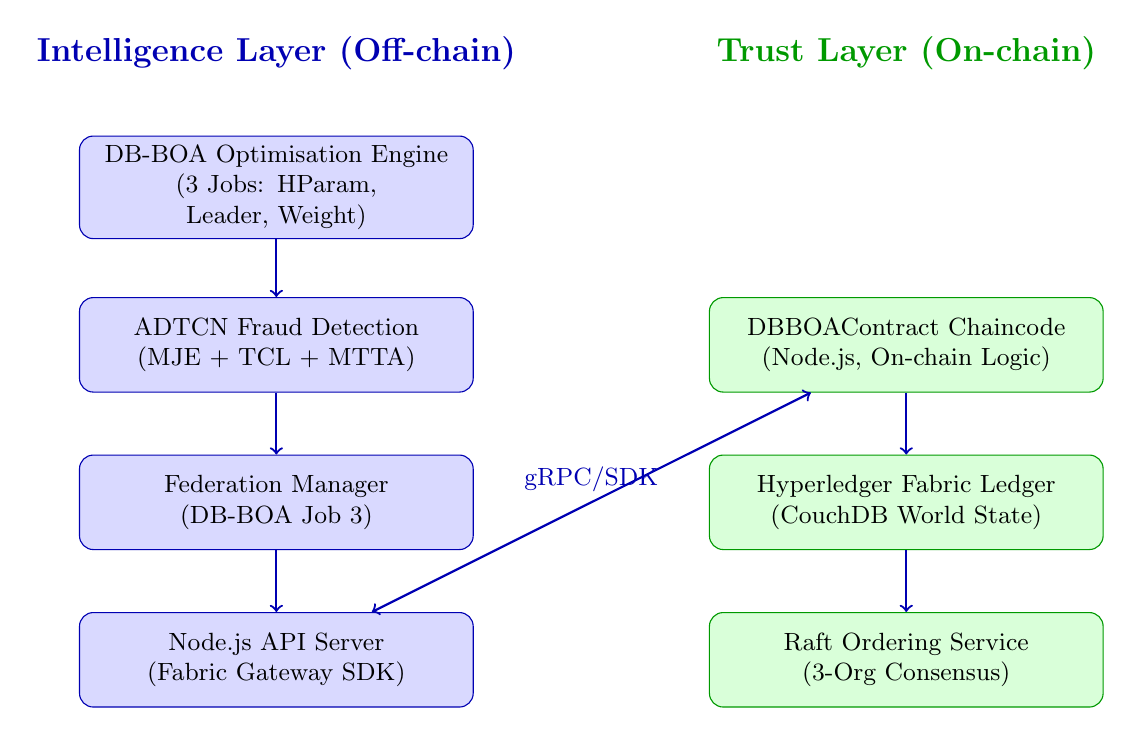
\begin{tikzpicture}[
  box/.style={
    rectangle, rounded corners=5pt, minimum width=5cm, minimum height=1.2cm,
    text centered, font=\small, text width=4.5cm, align=center
  },
  arrow/.style={->, thick, blue!70!black}
]
% Intelligence Layer (Left)
\node[box, fill=blue!15, draw=blue!70!black] (dbboa) at (0,8)
  {DB-BOA Optimisation Engine\\(3 Jobs: HParam, Leader, Weight)};
\node[box, fill=blue!15, draw=blue!70!black] (adtcn) at (0,6)
  {ADTCN Fraud Detection\\(MJE + TCL + MTTA)};
\node[box, fill=blue!15, draw=blue!70!black] (fedmgr) at (0,4)
  {Federation Manager\\(DB-BOA Job 3)};
\node[box, fill=blue!15, draw=blue!70!black] (apiserver) at (0,2)
  {Node.js API Server\\(Fabric Gateway SDK)};

% Trust Layer (Right)
\node[box, fill=green!15, draw=green!60!black] (chaincode) at (8,6)
  {DBBOAContract Chaincode\\(Node.js, On-chain Logic)};
\node[box, fill=green!15, draw=green!60!black] (ledger) at (8,4)
  {Hyperledger Fabric Ledger\\(CouchDB World State)};
\node[box, fill=green!15, draw=green!60!black] (ordering) at (8,2)
  {Raft Ordering Service\\(3-Org Consensus)};

% Layer Labels
\node[font=\large\bfseries, color=blue!70!black] at (0,9.7)
  {Intelligence Layer (Off-chain)};
\node[font=\large\bfseries, color=green!60!black] at (8,9.7)
  {Trust Layer (On-chain)};

% Arrows
\draw[arrow] (dbboa) -- (adtcn);
\draw[arrow] (adtcn) -- (fedmgr);
\draw[arrow] (fedmgr) -- (apiserver);
\draw[arrow, <->] (apiserver) -- (chaincode)
  node[midway, above, font=\small] {gRPC/SDK};
\draw[arrow] (chaincode) -- (ledger);
\draw[arrow] (ledger) -- (ordering);
\end{tikzpicture}
\caption{Two-Layer Architecture of the FL-ADTCN Framework. The Intelligence Layer (left) runs all non-deterministic computation off-chain in Python. The Trust Layer (right) records decisions and enforces incentive rules deterministically on Hyperledger Fabric.}
\label{fig:architecture_overview}
\end{figure}

\begin{table}[htbp]
\centering
\begin{tabular}{|p{3.5cm}|p{5.8cm}|p{5.8cm}|}
\hline
\textbf{Layer} & \textbf{What It Does} & \textbf{What It Does NOT Do} \\ \hline
\textbf{Intelligence Layer} (Python, off-chain) & Runs DB-BOA optimisation (Jobs 1, 2, 3); trains ADTCN; detects fraud; computes federation weights; generates all metrics and result plots. & Does not store data permanently; does not enforce incentive rules; does not communicate with peer institutions directly. \\ \hline
\textbf{Trust Layer} (Hyperledger Fabric, on-chain) & Records all Intelligence Layer decisions permanently; enforces incentive rules via chaincode; provides shared tamper-proof audit trail; distributes token rewards automatically. & Does not run DB-BOA; does not train ADTCN; does not detect fraud; does not make optimisation decisions. \\ \hline
\end{tabular}
\caption{Two-Layer Architecture: Responsibilities and Strict Boundaries}
\label{tab:architecture_layers}
\end{table}

\subsection{Intelligence Layer (Off-Chain)}

The Intelligence Layer is implemented in Python and runs on each institution's own computing infrastructure. It is responsible for all machine learning and optimisation computation:

\begin{itemize}
  \item \textbf{DB-BOA Optimisation Engine}: Executes all three DB-BOA optimisation jobs. Uses pseudo-random number generation and is therefore architecturally incompatible with on-chain execution (see Section~\ref{sec:determinism}).
  \item \textbf{ADTCN Model}: Trains and executes the fraud detection neural network on each institution's local transaction data. Raw data never leaves this layer.
  \item \textbf{Federation Manager}: Collects model weight vectors from all institutions, runs DB-BOA Job~3 to determine optimal aggregation weights, computes the weighted-average global model, and prepares the federation record for submission to the ledger.
  \item \textbf{Node.js API Server}: Provides a gRPC-based bridge between the Python Intelligence Layer and the Hyperledger Fabric Trust Layer, using the Fabric Gateway SDK to submit signed transactions.
\end{itemize}

\subsection{Trust Layer (On-Chain)}

The Trust Layer is the Hyperledger Fabric consortium blockchain. It is responsible for:

\begin{itemize}
  \item \textbf{State recording}: All decisions made by the Intelligence Layer — optimal hyperparameters, selected leader node, federation weights, fraud verdicts, consensus round outcomes — are written to the immutable ledger via chaincode invocations.
  \item \textbf{Rule enforcement}: The \texttt{DBBOAContract} chaincode encodes all incentive rules. When a fraud verdict is submitted, the chaincode automatically applies the appropriate token credit or debit. No human decision is involved.
  \item \textbf{Access control}: Every chaincode invocation is signed with the submitting organisation's X.509 certificate, issued by the Fabric Certificate Authority. The chaincode verifies the caller's identity before accepting any data.
  \item \textbf{Event emission}: The chaincode emits blockchain events — \texttt{FraudConfirmed}, \texttt{LeaderSelected}, \texttt{FederationCompleted} — which the API server subscribes to and forwards to a monitoring dashboard.
\end{itemize}

The Trust Layer does not run DB-BOA, does not train ADTCN, does not detect fraud, and does not make optimisation decisions. It records and enforces — nothing more.

\section{The Determinism Constraint}
\label{sec:determinism}

A critical architectural principle governs the boundary between the Intelligence Layer and the Trust Layer: the determinism constraint of Hyperledger Fabric chaincode. Given identical inputs, every endorsing peer in the Fabric network must produce exactly identical outputs. This is what makes consensus possible.

DB-BOA is a metaheuristic that uses pseudo-random number generation. Its execution path varies between runs — different peers running DB-BOA independently would reach different solutions, making endorsement consensus impossible. This is not a weakness of DB-BOA: the same constraint applies to Ethereum, Hyperledger Besu, Quorum, and every other blockchain platform. The correct and standard architecture for blockchain-AI systems is therefore exactly what this framework implements: computation off-chain, results on-chain.

Running DB-BOA off-chain and recording its outputs on-chain is not a compromise — it is the architecturally correct design. This is how JPMorgan's Liink, HSBC's FX settlement system, and IBM's Food Trust network all operate. The chaincode in this system implements no \texttt{Math.random()} calls in state-mutating functions and derives all timestamps from \texttt{ctx.stub.getTxTimestamp()} to ensure deterministic execution across all endorsing peers.

\section{Consortium Network Topology}

The consortium consists of three organisations modelling financial institutions:
\begin{itemize}
  \item \textbf{BankA (Org1MSP)}: The largest institution, holding 50\% of training data.
  \item \textbf{BankB (Org2MSP)}: The medium institution, holding 30\% of training data.
  \item \textbf{BankC (Org3MSP)}: The smallest institution, holding 20\% of training data. Used as the Byzantine attacker in adversarial testing.
\end{itemize}

The Fabric network consists of one peer per organisation (three peers total), one CA per organisation, and a single Raft ordering service node. The endorsement policy requires that at least two of the three organisations endorse a transaction before it is committed — a standard 2-of-3 majority policy resilient to one organisation being offline or malicious. All organisations maintain identical CouchDB world state replicas.

Figure~\ref{fig:consortium_topology} illustrates the physical network topology.

\begin{figure}[htbp]
\centering
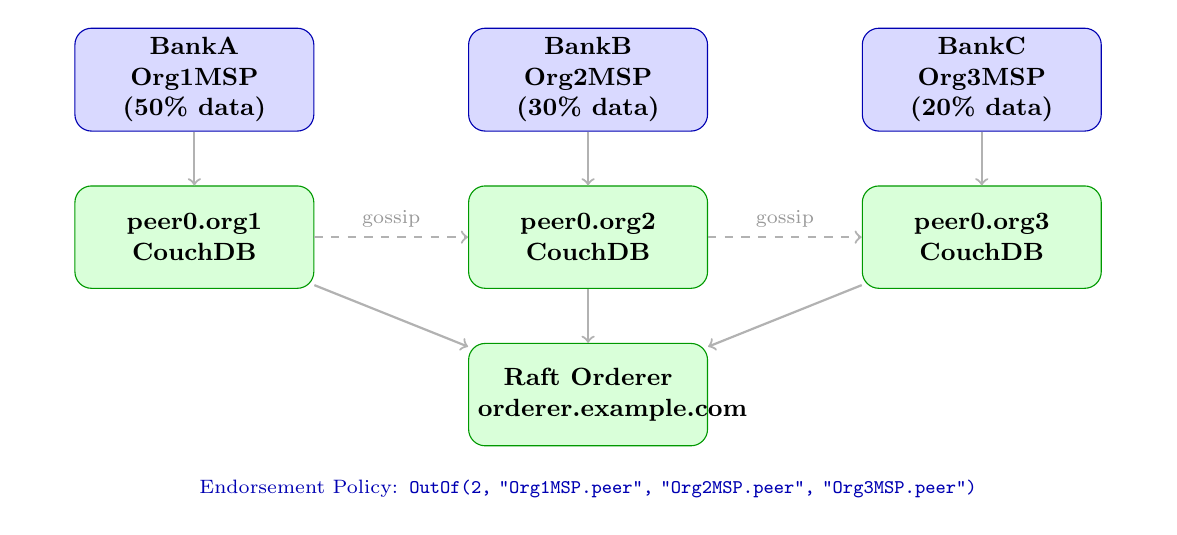
\begin{tikzpicture}[
  bank/.style={rectangle, rounded corners=6pt, minimum width=3.0cm, minimum height=1.3cm,
               text centered, font=\small\bfseries, fill=blue!15, draw=blue!70!black, text width=2.8cm},
  fabric/.style={rectangle, rounded corners=6pt, minimum width=3.0cm, minimum height=1.3cm,
                 text centered, font=\small\bfseries, fill=green!15, draw=green!60!black, text width=2.8cm},
  conn/.style={->, thick, gray!60},
  lbl/.style={font=\scriptsize, color=gray!80}
]
% Banks (top row)
\node[bank] (bA) at (0,4)   {BankA\\Org1MSP\\(50\% data)};
\node[bank] (bB) at (5,4)   {BankB\\Org2MSP\\(30\% data)};
\node[bank] (bC) at (10,4)  {BankC\\Org3MSP\\(20\% data)};

% Fabric peers (middle row)
\node[fabric] (pA) at (0,2) {peer0.org1\\CouchDB};
\node[fabric] (pB) at (5,2) {peer0.org2\\CouchDB};
\node[fabric] (pC) at (10,2){peer0.org3\\CouchDB};

% Raft orderer (bottom)
\node[fabric] (ord) at (5,0){Raft Orderer\\orderer.example.com};

% Bank → Peer (gRPC/SDK)
\draw[conn] (bA) -- (pA);
\draw[conn] (bB) -- (pB);
\draw[conn] (bC) -- (pC);

% Peers → Orderer
\draw[conn] (pA) -- (ord);
\draw[conn] (pB) -- (ord);
\draw[conn] (pC) -- (ord);

% Peer-to-peer gossip
\draw[conn, dashed] (pA) -- (pB) node[midway, above, lbl] {gossip};
\draw[conn, dashed] (pB) -- (pC) node[midway, above, lbl] {gossip};

% Endorsement policy
\node[font=\scriptsize, color=blue!70!black, text width=14cm, align=center] at (5,-1.2)
  {Endorsement Policy: \texttt{OutOf(2, "Org1MSP.peer", "Org2MSP.peer", "Org3MSP.peer")}};
\end{tikzpicture}
\caption{Consortium Network Topology. Three banking organisations each control one peer node and one Certificate Authority. Raft ordering service manages block production. The 2-of-3 endorsement policy ensures resilience to one offline or malicious organisation.}
\label{fig:consortium_topology}
\end{figure}

\section{Data Flow and Privacy Architecture}

\subsection{Privacy Principle}
Raw transaction data never leaves the institution that generated it. The only data that crosses institutional boundaries is:
\begin{itemize}
  \item Anonymised PCA-transformed feature vectors (30-dimensional numerical arrays, no personally identifiable information)
  \item Fraud detection verdicts (binary labels and probability scores)
  \item Model performance metrics (accuracy, MCC, sample counts)
  \item Neural network weight arrays (during federated rounds only)
  \item SHA-256 hashes of weight arrays (stored on-chain to prove integrity without exposing weights)
\end{itemize}

\subsection{PCA Anonymisation}

Before any transaction-related data is submitted to the blockchain, raw features are transformed using Principal Component Analysis (PCA) into a 30-dimensional numerical vector. This transformation is irreversible in practice: without the original PCA mapping — maintained privately by each institution — the vector cannot be traced back to a specific customer or transaction. This is the same approach used in the Kaggle ULB Credit Card Fraud Detection dataset, which serves as the empirical benchmark in this research.

\subsection{Cross-Institutional Verification Without Data Sharing}

When BankA submits a fraud detection result for transaction $\mathbf{x}$, Banks B and C verify by reading the anonymised feature vector from the blockchain, running it through their own locally-trained ADTCN, and submitting their own verdicts. Each institution thus runs its own independent model on the same anonymised features. No raw data is shared, no model is shared, and three independent verdicts are recorded. The chaincode determines consensus by majority (2-of-3). This mechanism achieves collaborative fraud detection without data exposure, satisfying the privacy requirements of GDPR, PCI-DSS, and the Bangladesh Bank Data Governance Policy.

\section{Off-Chain vs. On-Chain Boundary}

Table~\ref{tab:boundary} provides a precise specification of where each activity runs and why.

\begin{table}[htbp]
\centering
\caption{Precise Off-Chain vs. On-Chain Boundary}
\label{tab:boundary}
\begin{tabular}{|c|p{4.2cm}|p{4.0cm}|p{5.0cm}|}
\hline
\textbf{\#} & \textbf{Activity} & \textbf{Where it Runs} & \textbf{Reason} \\
\hline
1 & DB-BOA algorithm execution & Python, institution's machine & Non-deterministic; cannot run in chaincode \\
\hline
2 & ADTCN training and prediction & Python, institution's machine & Non-deterministic; private data involved \\
\hline
3 & Federation weight computation & Python, institution's machine & Non-deterministic optimisation \\
\hline
4 & Results written to ledger & Fabric chaincode, via SDK & Permanent, tamper-proof record \\
\hline
5 & Incentive rule enforcement & Fabric chaincode & Deterministic; rules agreed by all orgs \\
\hline
6 & Token balance management & Fabric chaincode & Neutral, trustless enforcement \\
\hline
7 & Audit trail and read access & Fabric ledger (CouchDB) & Shared, immutable, queryable \\
\hline
\end{tabular}
\end{table}
